\documentclass[twoside,10pt]{article}
%=================================================
% Basics
%=================================================
\usepackage{fixltx2e} % Makes \( \) equation style robust, among other
                      % things. Must be the first package.


% Makes ligatured fonts searchable and copyable in pdf readers
\usepackage{cmap} % Load before fontenc 

% Always include these font encodings in your document 
% unless you have a very good reason.
\usepackage[T1]{fontenc}
\usepackage[utf8]{inputenc}

\usepackage{verbatim}

%=============
% Fonts
%=============

\usepackage{lmodern} % Improved version of computer modern
\usepackage[scale=0.88]{tgheros} % Helvetica clone for sans serif font


\newcommand\hmmax{2} % Default is 3.
\newcommand\bmmax{2} % Default is 4.

\usepackage{bm} % boldmath must be called after the package
\providecommand{\mathbold}[1]{\bm{#1}}

%=============
% AMS Packages and fonts
%=============
\usepackage{amsmath,amsbsy,amsgen,amscd,amsthm,amsfonts,amssymb} 

%=============
% Margins and paper size
%=============
\usepackage[centering,top=1.5in,bottom=1.2in,left=1.4in,right=1.4in]{geometry}
\usepackage{parskip}


%=============
% Section headings
%=============
\usepackage[sf,bf,compact]{titlesec}

%=============
% Tables and lists
%=============
\usepackage{booktabs,longtable,tabu} % Nice tables
\setlength{\tabulinesep}{1mm}
\usepackage[font=small,margin=10pt,labelfont={sf,bf},labelsep={space}]{caption}

%=============
% Code output
%=============
% \usepackage{listings}
% \usepackage{minted}




\usepackage{enumitem}
\setitemize{itemsep=0pt} 
\setenumerate{itemsep=0pt}
\setlist{labelindent=\parindent,%  % Recommended by enumitem package
  font=\sffamily}


%=============
% Hyperlink colors
%=============
\usepackage[usenames,dvipsnames]{xcolor}
\definecolor{steelblue}{HTML}{A1BDC7}
\definecolor{orange}{HTML}{D98C21}
\definecolor{silver}{HTML}{B0ABA8}
\definecolor{rust}{HTML}{B8420F}
\definecolor{seagreen}{HTML}{2E6B69}
\definecolor{joshua}{HTML}{FBDC7F}
\definecolor{darksky}{HTML}{154c79}

\colorlet{steelblue}{silver!30!white}
\colorlet{darkorange}{orange!85!black}
\colorlet{darksilver}{silver!85!black}
\colorlet{darksteelblue}{steelblue!85!black}
\colorlet{darkrust}{rust!85!black}
\colorlet{darkseagreen}{seagreen!85!black}

\usepackage{url}
\usepackage[colorlinks=true]{hyperref}
\hypersetup{linkcolor=darkrust}    
\hypersetup{citecolor=darkseagreen}      
\hypersetup{urlcolor=darksilver}     

%=============
% Microtype
%=============
\usepackage[final]{microtype} 

%=====================
% Header
%=====================
% \usepackage{fancyhdr}
% \usepackage{nopageno} % Gets rid of page number at the bottom
% \fancyhf{} % Clear header style
% \renewcommand{\headrulewidth}{0.5pt} % remove the header rule
% \pagestyle{fancy}
% \fancyhead[LE,RO]{\textsf{\small \thepage}}
% 
% \setlength{\headheight}{14pt}
%=====================
% Fix delimiters
%=====================

% Fixes \left and \right spacing issues. See discussion at
% http://tex.stackexchange.com/questions/2607/spacing-around-left-and-right
\let\originalleft\left
\let\originalright\right
\renewcommand{\left}{\mathopen{}\mathclose\bgroup\originalleft}
\renewcommand{\right}{\aftergroup\egroup\originalright}

%=================================================
% Math macros
%=================================================

%=============
% Generalities
%=============
\usepackage{mathtools}
\mathtoolsset{centercolon}  % Makes := typeset correctly for definitions

%%% Equation numbering
%\numberwithin{equation}{section} 

%%% Annotations
\newcommand{\notate}[1]{\textcolor{red}{\textbf{[#1]}}}

%==============
% Symbols
%==============
\let\oldphi\phi
\let\oldeps\epsilon

\renewcommand{\phi}{\varphi}
\renewcommand{\epsilon}{\varepsilon}
\newcommand{\eps}{\varepsilon}

%==============
% Constants
%==============

% Set constants upright
\newcommand{\cnst}[1]{\mathrm{#1}}  
\newcommand{\econst}{\mathrm{e}}

\newcommand{\zerovct}{\vct{0}} % Zero vector
\newcommand{\Id}{\mathbf{I}} % Identity matrix
\newcommand{\onemtx}{\bm{1}}
\newcommand{\zeromtx}{\bm{0}}

%==============
% Sets
%==============
\providecommand{\mathbbm}{\mathbb} % In case we don't load bbm

% Reals, complex, naturals
\newcommand{\R}{\mathbbm{R}}
\newcommand{\C}{\mathbbm{C}}
\newcommand{\K}{\mathbbm{K}}
\newcommand{\N}{\mathbbm{N}}

%==============
% Probability
%==============
\newcommand{\Prob}{\operatorname{\mathbbm{P}}}
\newcommand{\Expect}{\operatorname{\mathbb{E}}}

%==============
% Vectors and matrices 
%==============
\newcommand{\vct}[1]{\mathbold{#1}}
\newcommand{\mtx}[1]{\mathbold{#1}}

\newcommand{\mrange}{\operatorname{range}}
\newcommand{\mnull}{\operatorname{null}}



\newcommand{\q}{\quad?\quad}

\begin{document}

\title{CSE 6643 Homework 2}
\author{Karl Hiner}
\date{}
\maketitle

\section{Less positive [12.5 pts]} 

Consider a symmetric positive definite matrix $\mtx{A}$ separated into subblocks according to
\begin{equation*}
  \mtx{A} = \begin{pmatrix}
    \mtx{A}_{1, 1} & \mtx{A}_{1, 2} \\
    \mtx{A}_{2, 1} & \mtx{A}_{2, 2}
  \end{pmatrix}.
\end{equation*}
Show that the matrix $\mtx{A}_{2,2} - \mtx{A}_{2,1} \mtx{A}_{1,1}^{-1} \mtx{A}_{1,2}$ is symmetric and positive definite. 

\quad First, note that $\mtx{A}_{2,2} - \mtx{A}_{2,1} \mtx{A}_{1,1}^{-1} \mtx{A}_{1,2}$ is the \textit{Schur complement} of $\mtx{A}$, which we will refer to as $\mtx{S}$ for brevity.
For $\mtx{S}$ to be symmetric, we must show that $\mtx{S}^T = \mtx{S}:$ 

\begin{align*}
\mtx{S}^T &= \left(\mtx{A}_{2,2} - \mtx{A}_{2,1} \mtx{A}_{1,1}^{-1} \mtx{A}_{1,2}\right)^T\\
&= \mtx{A}_{2,2}^T - \mtx{A}_{1,2}^T \left(\mtx{A}_{1,1}^{-1}\right)^T \mtx{A}_{2,1}^T \\
&= \mtx{A}_{2,2} - \mtx{A}_{2,1} \mtx{A}_{1,1}^{-1} \mtx{A}_{1,2} = \mtx{S}
\end{align*}

\quad Since $\mtx{A}$ is symmetric, $\mtx{A}_{1,2} = \mtx{A}_{2,1}^T$, $\mtx{A}_{2,1} = \mtx{A}_{1,2}^T$, and $\mtx{A}_{2,2} = \mtx{A}_{2,2}^T$.
Since $\mtx{A}$ is positive definite, it is invertible, and since it is symmetric, then its inverse is also symmetric, and $\left(\mtx{A}_{1,1}^{-1}\right)^T = \mtx{A}_{1,1}^{-1}$.
Thus, the above equality is satisfied and $\mtx{S}$ is symmetric.

To show that $\mtx{S}$ is positive definite, we need to show that for any non-zero vector $\vct{x}$, $\vct{x}^T \mtx{S} \vct{x} > 0$.

First, keeping in mind that $\mtx{A}_{2,1} = \left(\mtx{A}_{1,2}\right)^T$, let's define $\mtx{A}$ more compactly as:

\begin{equation*}
  \mtx{A} = \begin{pmatrix}
    \mtx{B} & \mtx{C} \\
    \mtx{C}^T & \mtx{D}
  \end{pmatrix}.
\end{equation*}

Then the Schur complement is $\mtx{S} = \mtx{D} - \mtx{C}^T \mtx{B}^{-1} \mtx{C}$, and we can express $\mtx{A}$ as

\begin{equation*}
  \mtx{A} = \begin{pmatrix}
    \mtx{I} & \mtx{0} \\
    \mtx{C}^T\mtx{B}^{-1} & \mtx{I}
  \end{pmatrix}
  \begin{pmatrix}
    \mtx{B} & \mtx{0} \\
    \mtx{0} & \mtx{S}
  \end{pmatrix}
  \begin{pmatrix}
    \mtx{I} & \mtx{B}^{-1}\mtx{C} \\
    \mtx{0} & \mtx{I}
  \end{pmatrix}
  =
  \mtx{N}
  \begin{pmatrix}
    \mtx{B} & \mtx{0} \\
    \mtx{0} & \mtx{S}
  \end{pmatrix}
  \mtx{N}^T.
\end{equation*}

$\mtx{N}$ is invertible, and its inverse can be found like an elementary real matrix, by negating its single off-diagonal element:

\begin{align*}
  \mtx{N} &=
  \begin{pmatrix}
    \mtx{I} & \mtx{0} \\
    \mtx{C}^T\mtx{B}^{-1} & \mtx{I}
  \end{pmatrix}\\
  \mtx{N}^{-1} &=
  \begin{pmatrix}
    \mtx{I} & \mtx{0} \\
    -\mtx{C}^T\mtx{B}^{-1} & \mtx{I}
  \end{pmatrix}
\end{align*}

Let $\mtx{M} \equiv \begin{pmatrix}
    \mtx{B} & \mtx{0} \\
    \mtx{0} & \mtx{S}
  \end{pmatrix}.$

Then,
\begin{align*}
  \mtx{M} &=
  \mtx{N}^{-1}\mtx{A}\left(\mtx{N}^{-1}\right)^T\\
  \vct{u}^T\mtx{M}\vct{u}
  &=
  \vct{u}^T\mtx{N}^{-1}\mtx{A}\left(\mtx{N}^{-1}\right)^T\vct{u} &\quad \text{(for any vector $\vct{u} \not\equiv \vct{0}$)}\\
  &=
  \vct{v}^T\mtx{A}\vct{v} &\quad (\vct{v} \equiv \left(\mtx{N}^{-1}\right)^T\vct{u})\\
  &> 0 &\quad \text{(since $\mtx{A}$ is positive definite)}
\end{align*}

Thus, $\mtx{M}$ is positive-definite.

Since $\mtx{A}$ is positive definite, then $\mtx{B}$ must be positive definite, since it is a principle submatrix of $\mtx{A}$ (and of $\mtx{M}$, which we just showed to also be positive definite!).

Thus, $\mtx{S} = \mtx{D} - \mtx{C}^T \mtx{B}^{-1} \mtx{C} = \mtx{A}_{2,2} - \mtx{A}_{2,1} \mtx{A}_{1,1}^{-1} \mtx{A}_{1,2}$ is also positive definite, since it is the other principle submatrix of the positive definite $\mtx{M}$.

\section{Just one [12.5 pts]}
Consider a matrix $\mtx{A} \in \R^{m \times m}$, with (unpivoted) LU-factorization given by $\mtx{A} = \mtx{L} \mtx{U}$. 
Propose an algorithm for computing the $(i, j)$-th entry of $\mtx{A}^{-1}$ using only $\mathcal{O}\left(\left(m + 1 - j\right)^2 + \left(m + 1 - i\right)^2\right)$ floating point operations. 

\begin{enumerate}
\item Compute the $j$-th column of $\mtx{A}^{-1}$ by solving $\mtx{L} \mtx{y} = \mtx{e}_j$ for $\mtx{y}$, where $\mtx{e}_j$ is the $j$-th standard basis vector.
This step takes $\mathcal{O}(\left(m + 1 - j\right)^2)$ operations.
\item Compute the $(i, j)$-th entry of $\mtx{A}^{-1}$ by solving $\mtx{U} \mtx{x} = \mtx{y}$ for $\mtx{x}$. Then the $i$-th entry of $\mtx{x}$ is the$(i, j)$-th entry of $\mtx{A}^{-1}$.
This step takes $\mathcal{O}(\left(m + 1 - i\right)^2)$ operations.
\end{enumerate}

\quad The total number of operations is $\mathcal{O}(\left(m + 1 - j\right)^2 + \left(m + 1 - i\right)^2)$.

\section{SVD [25 pts]}
In class, we have reminded ourselves of the SVD of square matrices. 
Use the recommended literature from the class syllabus to catch up on the SVD applied to non-square matrices. 

We denote as $\sigma_{\mathrm{min}}$ and $\sigma_{\mathrm{max}}$ the smallest and largest singular value of a matrix and by $\lambda_{i}$ its $i$-th eigenvalue. 
We consider general matrices $\mtx{A} \in \R^{m \times n}$ and $\mtx{B} \in \R^{n \times l}$.
Show that the following results hold 

\subsection*{(a) [5 pts]}
  \begin{equation*}
    \sigma_{\mathrm{max}}(\mtx{A}) \|\vct{x}\|_2 \geq \|\mtx{A} \vct{x}\|_2, \forall \vct{x} \in \R^n
  \end{equation*}

\begin{align*}
 \|\mtx{A} \vct{x}\|_2 &\leq \|\mtx{A}\|_2\|\vct{x}\|_2 &\quad\text{(consistency of $\|\cdot\|_2$ operator norm with induced vector norm)}\\
 &= \sigma_{\mathrm{max}}(\mtx{A})\|\vct{x}\|_2 &\quad\text{(Thm. 5.3 in Trefethen \& Bau: $\|\mtx{A}\|_2 = \sigma_{\mathrm{max}}(\mtx{A})$)}
\end{align*}

\subsection*{(b) [5 pts]}
  \begin{equation*}
    m \geq n \Rightarrow \|\mtx{A}\vct{x}\|_2 \geq \sigma_{\mathrm{min}}\left(\mtx{A}\right) \|\vct{x}\|_2, \forall \vct{x} \in \R^n
  \end{equation*}

\begin{align*}
  \dfrac{\vct{x}^{*}\mtx{A}^{*}\mtx{A}\vct{x}}{\|\vct{x}\|_2^2} &\geq\inf \limits_{\vct{y} \in \R^m \setminus \{\vct{0}\}} \dfrac{\vct{y}^{*} \mtx{A}^{*}\mtx{A}\vct{y}}{\|\vct{y}\|_2^2} &\text{($\forall\vct{x} \in \R^n$)}\\
  \vct{x}^{*}\mtx{A}^{*}\mtx{A}\vct{x} &\geq \left(\inf \limits_{\vct{y} \in \R^m \setminus \{\vct{0}\}} \dfrac{\vct{y}^{*} \mtx{A}^{*}\mtx{A}\vct{y}}{\|\vct{y}\|_2^2}\right) \|\vct{x}\|_2^2  &\text{(multiply both sides by $\|\vct{x}\|_2^2$)}\\
  \vct{x}^{*}\mtx{A}^{*}\mtx{A}\vct{x} &\geq \lambda_{\mathrm{min}}(\mtx{A}^{*}\mtx{A}) \|\vct{x}\|_2^2 &\text{$\left(\lambda_{\mathrm{min}}\left(\mtx{A}\right) = \inf \limits_{\vct{y} \in \R^m \setminus \{\vct{0}\}} \dfrac{\vct{y}^{*} \mtx{A}\vct{y}}{\|\vct{y}\|_2^2}\right)$}\\
  \|\mtx{A}\vct{x}\|_2^2 &\geq \lambda_{\mathrm{min}}(\mtx{A}^{*}\mtx{A}) \|\vct{x}\|_2^2 &\text{($\|\vct{v}\|_2 = \sqrt{\vct{v}^{*}\vct{v}}$)}\\
  \|\mtx{A}\vct{x}\|_2 &\geq \sqrt{\lambda_{\mathrm{min}}(\mtx{A}^{*}\mtx{A})} \|\vct{x}\|_2 &\text{(take square root of both sides)}\\
  &=\sigma_{\mathrm{min}}\left(\mtx{A}\right) \|\vct{x}\|_2 &\text{(def. of singular values)}\\
\end{align*}

\subsection*{(c) [5 pts]}
  \begin{equation*}
    m = n \Rightarrow \sigma_{\mathrm{min}}(\mtx{A}) \leq \left|\lambda_{i}\left(\mtx{A}\right)\right| \leq \sigma_{\mathrm{max}}\left(\mtx{A}\right), \forall i 
  \end{equation*}

  Let $\lambda_i$ be an eigenvalue of $\mtx{A}$, and let $\vct{v_i}$ be a corresponding unit eigenvector such that $\mtx{A}\vct{v_i} = \lambda_i\vct{v_i}$. 
  Taking the 2-norm of both sides:
  \begin{align*}
    \|\mtx{A}\vct{v_i}\|_2 &= \|\lambda_i \vct{v_i}\|_2\\
    &= |\lambda_i| \|\vct{v_i}\|_2\\
    &= |\lambda_i|\quad\quad\quad\text{(since $\|\vct{v_i}\|_2 = 1$)}
  \end{align*}

  Also, note that since $\mtx{A}$ is square when $m = n$, $\mtx{A}^{*}\mtx{A}$ is positive semidefinite, and can thus be decomposed into $\mtx{U}\mtx{\Lambda}\mtx{U}^{*}$, where $\mtx{\Lambda}$ is an $mxm$ diagonal matrix whose entries are the eigenvalues of $\mtx{A}^{*}\mtx{A}$.

  So then,
  \begin{align*}
    |\lambda_{\mathrm{min}}| &= \|\mtx{A}\vct{v}_{\mathrm{min}}\|_2&\quad\text{(let $\vct{v}_{\mathrm{min}}$ be a unit e.v. of $\mtx{A} \to \lambda_{\mathrm{min}}$)}\\
    |\lambda_{\mathrm{min}}|^2 &= \|\mtx{A}\vct{v}_{\mathrm{min}}\|_2^2&\quad\text{(squaring both sides)}\\
    &= \vct{v}_{\mathrm{min}}^{*}\mtx{A}^{*}\mtx{A}\vct{v}_{\mathrm{min}}&\quad\text{(def. of vector 2-norm)}\\
    &\geq \inf_{\|\vct{x}\| = 1}{\vct{x}^{*}\mtx{A}^{*}\mtx{A}\vct{x}}&\quad\text{(since $\vct{v}_{\mathrm{min}}$ is min. eigenvalue)}\\
    &= \inf_{\|\vct{x}\| = 1}{\vct{x}^{*}\mtx{U}\mtx{\Lambda}\mtx{U}^{*}\vct{x}}&\quad\text{($\mtx{\Lambda}_{i,i} = \lambda_i(\mtx{A}^{*}\mtx{A})$)}\\
    &= \inf_{\|\vct{y}\| = 1}{\vct{y}^{*}\mtx{\Lambda}\vct{y}}&\quad\text{(let $\vct{y} \equiv \mtx{U}^{*}\vct{x}$)}\\
    &= \lambda_{\mathrm{min}}(\mtx{A}^{*}\mtx{A})&\quad\text{(def. of $\lambda_{\mathrm{min}}$ - see (4) below)}\\
    &= \sigma_{\mathrm{min}}(\mtx{A})^2&\quad\text{(def. of singular value)}\\
  \end{align*}

  Thus, $|\lambda_{\mathrm{min}}(\mtx{A})|^2 \geq \sigma_{\mathrm{min}}(\mtx{A})^2 \implies |\lambda_{\mathrm{min}}(\mtx{A})| \geq \sigma_{\mathrm{min}}(\mtx{A})$.

  The same argument can be applied to show that $|\lambda_{\mathrm{max}}(\mtx{A})| \leq \sigma_{\mathrm{max}}(\mtx{A})$, which shows that
  \begin{equation*}
    m = n \Rightarrow \sigma_{\mathrm{min}}(\mtx{A}) \leq \left|\lambda_{i}\left(\mtx{A}\right)\right| \leq \sigma_{\mathrm{max}}\left(\mtx{A}\right), \forall i 
  \end{equation*}

\subsection*{(d) [5 pts]}
  \begin{equation*}
    \sigma_{\mathrm{max}}\left(\mtx{A}\right) = 1 / \sigma_{\mathrm{min}}\left(\mtx{A}^{-1}\right)\text{, if $\mtx{A}^{-1}$ exists}
  \end{equation*}

  We can decompose any matrix $\mtx{A} \in \R^{mxn}$ into components $\mtx{A} = \mtx{U} \mtx{\Sigma} \mtx{V}^T$, where $\mtx{U}$ and $\mtx{V}^T$ are orthogonal, and $\mtx{\Sigma} \in \R^{mxn}$ is a diagonal matrix whose entries $\mtx{\Sigma}_{i,i}$ contain all of the singular values of $\mtx{A}$.
  Since $\mtx{A}$ is invertible, all of its singular values will be nonzero, and so $\mtx{\Sigma}_{i,i} \neq 0, \forall i$.

  If we invert both sides of this equality, we get $\mtx{A}^{-1} = \mtx{V} \mtx{\Sigma}^{-1} \mtx{U}^T$, which holds since we are given that $\mtx{A}^{-1}$ exists.
  $\mtx{\Sigma}^{-1}$ also exists, since it is a diagonal matrix with no zeros on its diagonal.
  Its (also nonzero) diagonal entries are the singular values of $\mtx{A}^{-1}$, and its inverse can be found by inverting each of its diagonal elements (a property not proven here):

  \begin{align*}
    \mtx{\Sigma} &=
    \begin{bmatrix}
      \sigma_{1}(\mtx{A}) &  & \\ 
      & \ddots & \\ 
      &  & \sigma_{n}(\mtx{A})\\
      & \dots
    \end{bmatrix}\\
    \mtx{\Sigma}^{-1} &=
    \begin{bmatrix}
      \dfrac{1}{\sigma_{1}(\mtx{A})} &  & \\ 
      & \ddots & \\ 
      &  & \dfrac{1}{\sigma_{n}(\mtx{A})}\\
      & \dots
    \end{bmatrix}.
  \end{align*}

  Thus, for any $1 \leq i \leq n$, $\sigma_i(\mtx{A}) = \mtx{\Sigma}_{i,i} = \dfrac{1}{(\mtx{\Sigma}^{-1})_{i,i}} = \dfrac{1}{\sigma_i(\mtx{A}^{-1})}$.

  Finally, let $j = \arg\!\max\limits_{i}{\Sigma_{i,i}}$.
  Then $\sigma_j(\mtx{A}) = \sigma_{\mathrm{max}}(\mtx{A})$.
  Since each element in $\Sigma^{-1}$ is inverted, $j = \arg\!\min\limits_{i}{(\Sigma^{-1})_{i,i}}$, and so $\sigma_j(\mtx{A}^{-1}) = \sigma_{\mathrm{min}}(\mtx{A}^{-1})$, and so $\sigma_{\mathrm{max}}\left(\mtx{A}\right) = \dfrac{1}{\sigma_{\mathrm{min}}\left(\mtx{A}^{-1}\right)}$.

\subsection*{(e) [5 pts]}
  \begin{equation*}
    \text{Find the most general conditions on $m$, $n$, and $l$, under which } \sigma_{\mathrm{min}}\left(\mtx{A}\mtx{B}\right) \geq \sigma_{\mathrm{min}}\left(\mtx{A}\right) \sigma_{\mathrm{min}}\left(\mtx{B}\right).
  \end{equation*}

  If both $\mtx{A}$ and $\mtx{B}$ are positive semi-definite, then the inequality holds.

  The product of two positive semi-definite matrices is always positive semi-definite, and so its eigenvalues are non-negative.
  Thus, the smallest eigenvalue of the product is $\geq 0$, and the product of the smallest eigenvalues of the matrices is also $\geq 0$.

  Thus, the smallest eigenvalue of the product is $\geq$ the product of the smallest eigenvalues of the two positive semi-definite matrices.

\section{Inverses [25 pts]}
We consider $\mtx{A} \in \R^{m \times m}$ and assume that $\mtx{A}^{-1}$ exists. 
You may use without proof that if $\mtx{A}$ is symmetric, its largest and smallest eigenvalues are characterized as 
\begin{equation*}
   \lambda_{\mathrm{max}}\left(\mtx(A)\right) = \sup \limits_{\vct{x} \in \R^m \setminus \{\vct{0}\}} \frac{\vct{x}^T \mtx{A}\vct{x}}{\|\vct{x}\|_2^2}
\end{equation*}
and 
\begin{equation*}
   \lambda_{\mathrm{min}}\left(\mtx(A)\right) = \inf \limits_{\vct{x} \in \R^m \setminus \{\vct{0}\}} \frac{\vct{x}^T \mtx{A}\vct{x}}{\|\vct{x}\|_2^2}
\end{equation*}


\subsection*{(a) [5 pts]}
Show that 
\begin{equation}
  \left\|\mtx{A}^{-1}\right\|_2^{-1} = \inf \limits_{\vct{x} \in \R^m \setminus \{\vct{0}\}} \frac{\|\mtx{A}\vct{x}\|_2}{\|\vct{x}\|_2}
\end{equation}

\begin{align*}
  \mtx{A} &= \mtx{U} \mtx{\Sigma} \mtx{V}^T&\quad\text{(SVD decomposition of $\mtx{A}$)}\\
  \mtx{A}^{-1} &= \mtx{V} \mtx{\Sigma}^{-1} \mtx{U}^T&\quad\text{(invert both sides)}\\
  \left\|\mtx{A}^{-1}\right\|_2 &= \left\|\mtx{V} \mtx{\Sigma}^{-1} \mtx{U}^T\right\|_2&\quad\text{(take the 2-norm of both sides)}\\
  &= \sigma_{\mathrm{max}}\left(\mtx{V} \mtx{\Sigma}^{-1} \mtx{U}^T\right)&\quad\text{(since $\left\|\mtx{B}\right\|_2 = \sigma_{\mathrm{max}}\left(\mtx{B}\right)$ for any matrix $\mtx{B}$)}\\
  &= \sigma_{\mathrm{max}}\left(\mtx{\Sigma}^{-1}\right)&\quad\text{(since $\mtx{V}$ and $\mtx{U}$ are orthogonal)}\\
  &= \frac{1}{\sigma_{\mathrm{min}}\left(\mtx{\Sigma}\right)}&\quad\text{((3d) above)}\\
  &= \frac{1}{\sigma_{\mathrm{min}}\left(\mtx{A}\right)}&\quad\text{(def. of $\mtx{\Sigma}$)}\\
  \left\|\mtx{A}^{-1}\right\|_2^{-1} &= \sigma_{\mathrm{min}}\left(\mtx{A}\right)&\quad\text{(invert both sides)}\\
  &=  \inf \limits_{\vct{x} \in \R^m \setminus \{\vct{0}\}} \frac{\|\mtx{A}\vct{x}\|_2}{\|\vct{x}\|_2}&\quad\text{(def. of $\sigma_\mathrm{min}$)}
\end{align*}

\subsection*{(b) [5 pts]}
Show that 
\begin{equation}
  \left\|\mtx{A}^{-1}\right\|_2^{-1} \geq \inf \limits_{\vct{x} \in \R^m \setminus \{\vct{0}\}} \frac{|\vct{x}^T \mtx{A}\vct{x}|}{\|\vct{x}\|_2^2}
\end{equation}

\begin{align*}
  \left\|\mtx{A}^{-1}\right\|_2^{-1} &= \inf \limits_{\vct{x} \in \R^m \setminus \{\vct{0}\}} \frac{\|\mtx{A}\vct{x}\|_2}{\|\vct{x}\|_2}&\quad\text{(from above)}\\
  &= \inf \limits_{\vct{x} \in \R^m \setminus \{\vct{0}\}} \frac{\|\mtx{A}\vct{x}\|_2\|\vct{x}\|_2}{\|\vct{x}\|_2^2}&\quad\text{(multiply num. and dem. by $\|\vct{x}\|_2$)}\\
  &= \inf \limits_{\vct{x} \in \R^m \setminus \{\vct{0}\}} \frac{\|\vct{x}^T \mtx{A}\vct{x}\|_2}{\|\vct{x}\|_2^2}&\quad\text{($\|\vct{x}^T \mtx{A}\vct{x}\|_2 = \|\mtx{A}\vct{x}\|_2 \|\vct{x}\|_2$)}\\
  &\geq \inf \limits_{\vct{x} \in \R^m \setminus \{\vct{0}\}} \frac{|\vct{x}^T \mtx{A}\vct{x}|}{\|\vct{x}\|_2^2}&\quad\text{($|\vct{x}^T \mtx{A}\vct{x}| \le \|\vct{x}^T \mtx{A}\vct{x}\|_2$)}
\end{align*}

\subsection*{(c) [5 pts]}

Show that for symmetric matrices $\mtx{M}, \mtx{N} \in \R^{m \times m}$, 
\begin{equation}
  \lambda_{\mathrm{min}}(\mtx{M} + \mtx{N}) \geq \lambda_{\mathrm{min}}\left(\mtx{M}\right) + \lambda_{\mathrm{min}}\left(\mtx{N}\right)
\end{equation}

To start, we will substitute the given expression for $\lambda_{\mathrm{min}}$, $\lambda_{\mathrm{min}}\left(\mtx{A}\right) = \inf \limits_{\vct{x} \in \R^m \setminus \{\vct{0}\}} \dfrac{\vct{x}^T \mtx{A}\vct{x}}{\|\vct{x}\|_2^2}$, for the left-side term, $\lambda_{\mathrm{min}}(\mtx{M} + \mtx{N})$:

\begin{align*}
  \lambda_{\mathrm{min}}(\mtx{M} + \mtx{N}) &= \inf \limits_{\vct{x} \in \R^m \setminus \{\vct{0}\}} \dfrac{\vct{x}^T \left(\mtx{M} + \mtx{N}\right)\vct{x}}{\|\vct{x}\|_2^2}\\
  &= \inf \limits_{\vct{x} \in \R^m \setminus \{\vct{0}\}} \dfrac{\vct{x}^T \mtx{M}\vct{x} + \vct{x}^T\mtx{N}\vct{x}}{\|\vct{x}\|_2^2}\\
  &= \inf \limits_{\vct{x} \in \R^m \setminus \{\vct{0}\}} \left(\dfrac{\vct{x}^T \mtx{M}\vct{x} }{\|\vct{x}\|_2^2} + \dfrac{\vct{x}^T\mtx{N}\vct{x}}{\|\vct{x}\|_2^2}\right)\\
\end{align*}

Next, restate the given left- and right-side terms, using an unknown inequality, "$?$", as a placeholder:

\begin{align*}
  \lambda_{\mathrm{min}}(\mtx{M} + \mtx{N}) &\q \lambda_{\mathrm{min}}\left(\mtx{M}\right) + \lambda_{\mathrm{min}}\left(\mtx{N}\right)\\
  \inf \limits_{\vct{x} \in \R^m \setminus \{\vct{0}\}} \left(\dfrac{\vct{x}^T \mtx{M}\vct{x} }{\|\vct{x}\|_2^2} + \dfrac{\vct{x}^T\mtx{N}\vct{x}}{\|\vct{x}\|_2^2}\right) &\q  \inf \limits_{\vct{y} \in \R^m \setminus \{\vct{0}\}} \left(\dfrac{\vct{y}^T \mtx{M}\vct{y}}{\|\vct{y}\|_2^2}\right) + \inf \limits_{\vct{z} \in \R^m \setminus \{\vct{0}\}} \left(\dfrac{\vct{z}^T \mtx{N}\vct{z}}{\|\vct{z}\|_2^2}\right)\\
\end{align*}

To determine what the unknown inequality, "$?$", must be, we observe that the left side is the \text{same expression} as the right side, except that it is optimizing to find a \textit{single} infimum value for both terms, while the right side is jointly optimizing for \textit{two separate} infimums - one for each term.
Another way of thinking about this is that the right side is \textit{less constrained} than the left in its "search" for a minimum (real) value - its "search space" is a superset of that of the left side, since it's allowed to test different vectors $\vct{y}$ and $\vct{z}$ on the left and right terms, respectively, rather than being constrained to test the same $\vct{y} = \vct{z}$ as the left side is.

Also, note that this unknown inequality "$?$", must allow for the case of equivalence, for example when $\mtx{M} = \mtx{N}$.

Although this argument is hand wavy, I hope that it is sufficient to convince the reader (grader), that the inequality "$?$" must be "$\geq$".

\subsection*{(d) [5 pts]}
In the same setting as (c), show that 
\begin{equation}
  \lambda_{\mathrm{max}}(\mtx{M} + \mtx{N}) \leq \lambda_{\mathrm{max}}\left(\mtx{M}\right) + \lambda_{\mathrm{max}}\left(\mtx{N}\right)
\end{equation}

Using the same approach as (c), we substitute the given expression for $\lambda_{\mathrm{max}}$,

\begin{equation*}
   \lambda_{\mathrm{max}}\left(\mtx{A}\right) = \sup \limits_{\vct{x} \in \R^m \setminus \{\vct{0}\}} \frac{\vct{x}^T \mtx{A}\vct{x}}{\|\vct{x}\|_2^2},
\end{equation*}

and determine the unknown inequality, "$?$":

\begin{align*}
  \lambda_{\mathrm{max}}(\mtx{M} + \mtx{N}) &\q \lambda_{\mathrm{max}}\left(\mtx{M}\right) + \lambda_{\mathrm{max}}\left(\mtx{N}\right)\\
  \sup \limits_{\vct{x} \in \R^m \setminus \{\vct{0}\}} \left(\dfrac{\vct{x}^T \mtx{M}\vct{x} }{\|\vct{x}\|_2^2} + \dfrac{\vct{x}^T\mtx{N}\vct{x}}{\|\vct{x}\|_2^2}\right) &\q  \sup \limits_{\vct{y} \in \R^m \setminus \{\vct{0}\}} \left(\dfrac{\vct{y}^T \mtx{M}\vct{y}}{\|\vct{y}\|_2^2}\right) + \sup \limits_{\vct{z} \in \R^m \setminus \{\vct{0}\}} \left(\dfrac{\vct{z}^T \mtx{N}\vct{z}}{\|\vct{z}\|_2^2}\right)\\
\end{align*}

Using the exact same argument as above, but noting that the functions being optimized here are supremums instead of infimums, this inequality "$?$" must be "$\leq$".

\subsection*{(e) [5 pts]}
For $\mtx{A}$ symmetric positive definite, show that 
\begin{equation*}
  \|\mtx{A}^{-1}\|_{2}^{-1} = \inf \limits_{\vct{x} \in \R^m \setminus \{\vct{0}\}} \frac{\vct{x}^T \mtx{A} \vct{x}}{\|\vct{x}\|^2_2}
\end{equation*}

In (4a) above, we showed that 

\begin{equation*}
  \left\|\mtx{A}^{-1}\right\|_2^{-1} = \sigma_{\mathrm{min}}\left(\mtx{A}\right).
\end{equation*}

Since 

\begin{equation*}
  \lambda_{\mathrm{min}}\left(\mtx(A)\right) = \inf \limits_{\vct{x} \in \R^m \setminus \{\vct{0}\}} \frac{\vct{x}^T \mtx{A}\vct{x}}{\|\vct{x}\|_2^2},
\end{equation*}

and since, for symmetric positive definite matrices, the minimum singular value is equal to the minimum eigenvalue, we are done.

(The singular values are equal to the square roots of the eigenvalues, and the eigenvalues for a symmetric positive definite matrix are all positive.)

\section{Oblivion [25 pts]}
\subsection*{(c) [5 pts]}
Use section \texttt{HW2\_driver.jl} to try the performance of the blocked algorithm for different matrix sizes and block sizes. 
Describe your results, and for the most interesting set of parameters, hand in the resulting plot with your homework.
Describe and explain the results.

\quad I found that, for the default settings, I found that the block size mattered a great deal, with times increasing as block sizes increased after about 512-1024.

However, I found that the absolute performance for large matrix sizes was relatively poor, and improved a great deal by making all matrix sizes the same size, and making them powers of two.
This is likely because the matrices are then all evenly divided into the power-of-two block sizes, as well as perhaps allowing for more contiguous memory access if the powewr-of-two blocks fits well inside the cache.

Shown in the plot below in Fig. 1 is an experiment with all matrix sizes equal to 2048.
Here, we can see that performance first improves with increaes block size, until block size exceeds 512, and then maxes out when the block size equals the matrix size.
This likely corresponds to the blocks fitting inside the cache evenly at these smaller power-of-two block sizes.

\begin{figure}[htb]
  \begin{center}
  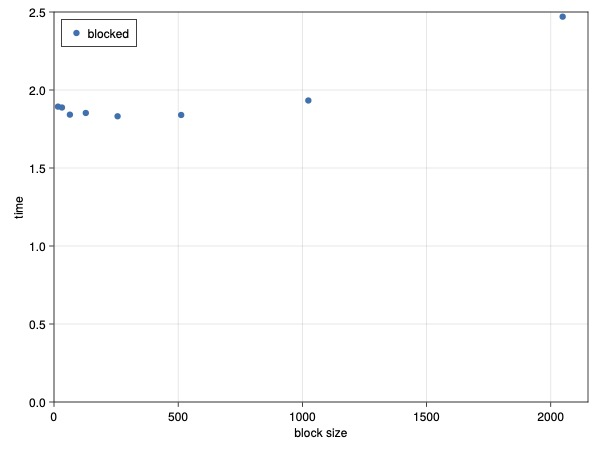
\includegraphics[width=150mm]{HW2_code/performance_blocked_2048.jpg}
  \end{center}
  \caption{All matrices length 2048}
  \label{fig:figure1}
  \end{figure}
  

\subsection*{(e) [5 pts]} Use part (e) of \texttt{HW2\_driver.jl} to benchmark your new algorithm for different values of \texttt{bks}. 
Are you able to obtain an improvement over the blocked algorithm? 
Hand in the figure produced by part (e) of \texttt{HW2\_driver.jl} for what you consider the most interesting set of parameters.
Algorithms of this type are called ``cache-oblivious.'' 
Explain why this is the case and what could be the theoretical advantages of this particular cache-oblivious algorithm.

As shown in Fig. 2 below, I was able to obtain a performance improvement for all but the smallest block sizes.

Cache-oblivious methods take advantage of the hierarchical nature of modern memory systems, which have multiple cache levels.
By working with progressively smaller problem sizes, it allows for taking advantage of the different cache sizes within this memory hierarchy.
The operating system can potentially better optimize cache utilization and memory access patterns with multiple problem sizes, rather than working with only a single fixed size.

For very small block sizes, the operating system will have fewer opportunities to take advantage of varying problem sizes, which explains my results.

\begin{figure}[htb]
  \begin{center}
  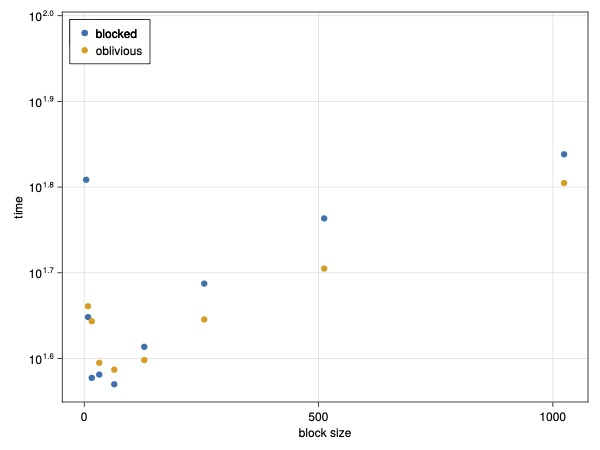
\includegraphics[width=150mm]{HW2_code/performance_blocked_and_oblivious.jpg}
  \end{center}
  \caption{All matrices length 2048}
  \label{fig:figure2}
  \end{figure}
  
% 
% \subsection*{(b) Matrix-vector-multiplication [5 pts]} 
% Complete the function \texttt{u\_is\_A\_times\_v!(u, A, v)} in \texttt{HW1\_your\_code.jl} that overwrites the input vector \texttt{u} with the product of the input matrix \texttt{A} and the input vector \texttt{v}.
% 
% \subsection*{(c) Matrix-matrix-multiplication [5 pts]} 
% Complete the function \texttt{A\_is\_B\_times\_C!(A, B, C)} in \texttt{HW1\_your\_code.jl} that overwrites the input matrix \texttt{A} with the product of the input matrices \texttt{B} and \texttt{C}.
% 
% \subsection*{(d) Testing [5 pts]}
% From the directory \texttt{HW1\_CODE}, run the command 
% \begin{verbatim}
%   julia --project=. HW1_driver.jl
% \end{verbatim}
% to test your code. Here, the \texttt{-\,-\,project=.} tells Julia to use \texttt{Manifest.toml} and \texttt{Project.toml} determine which version (if any) of packages to use.
% Make sure that your code passes all \texttt{@assert} statements, which test your functions against Julia's built-in functions.
% 
% \subsection*{(e) Optimization [5 pts]} 
% Make sure that your code does not allocate any memory, as evidenced by the \texttt{@btime} calls in \texttt{HW1\_driver.jl} returning \texttt{(0\,allocations:\,0\,bytes)}.
% This is important for performance reasons since allocating memory may be orders of magnitudes slower than floating-point arithmetic. 
% Now try reordering the for-loops in your implementations from parts (a) and (b) and observe the resulting timings provided by \texttt{@btime}. 
% Which order leads to the best and worst performance? 
% What are the corresponding wall-clock times as measured by \texttt{@btime}? 

















%\bibliographystyle{plain}
%\bibliography{temp,externalPapers,groupPapers}

\end{document}
